\chapter{Quantum Chromodynamics}
\label{chap:QCD}

The strong interaction is the fundamental force responsible for binding quarks together into hadrons. It is described by \ac{QCD} which is a gauge theory based on $SU(3)_{C}$ symmetry. One of the key features of \ac{QCD} is the phenomenon known as asymptotic freedom, namely strong force weakens at shorter distance. This property differentiates the strong force with all three other fundamental forces. A brief description of the formulation of \ac{QCD} is given in \autoref{sec:QCD}. Asymptotic freedom predicts that the strong coupling constant, denoted by $\alpha_{S}$, is small at short distance, which allows for perturbative expansion of the probability amplitude. However, the expansion parameter $\alpha_{S}$ at long distance becomes too large and the predictions are therefore no longer reliable. Techniques developed to model \ac{QCD} phenomenon in this regime are collectively known as nonperturbative-\ac{QCD}, which is discussed in \autoref{sec:Collision}.

\section{Formulation of QCD}
\label{sec:QCD}

The modern theory of strong interaction started in 1964 when the quark model was independently proposed by American physicists George Zweig~\cite{Zweig:1964ruk} and his Ph.D. advisor Murray Gell-Mann~\cite{Gell-Mann:1964ewy}. The original objective of this model was to explain the spectrum of new hadrons discovered at rapid speed at the time. In this early version, mesons and baryons were viewed as composite objects formed by spin-$\frac{1}{2}$ particles, named ``quarks'' by Gell-Mann and ``aces'' by Zweig, They came with several quantum charges and three different flavors: $u$, $d$, $s$. The strange quarks in this model had a higher mass, which explained the mass differences between different baryons and mesons.

This model was successful in explaining why protons of same charge were bound together -- they were bound states of more fundamental particles affected by the strong interactions. However, gaps still existed in this model, mostly notably the tension with Fermi-Dirac statistics. It was indicated by this model that the wave function for $\Omega^{-}$ (sss) should be symmetrical in the interchange of strange quarks. However, the wave function must be antisymmetric because quarks had half spins in this model. Gell-Mann and his collaborations was able resolve this problem in early 1970s by introducing color charges~\cite{Fritzsch:1973pi}. Under this updated framework, each flavor of quark should come with three colors, namely red, green, and blue. The wave functions of hadrons were assumed to be singlets of the gauge group $SU(3)_{C}$. For example, the wave function for $\Omega^{-}$ meson can be represented as,

\begin{equation}
(sss)\rightarrow(s_{r}s_{g}s_{b}-s_{g}s_{r}s_{b}+s_{b}s_{r}s_{g}-s_{r}s_{b}s_{g}+s_{g}s_{b}s_{r}-s_{b}s_{g}s_{r}),
\end{equation}

which restored the Fermi-Dirac statistics.  

The force mediators in this theory, known as ``gluons'', also carry color charges. This enables gluon-gluon self-interaction. The \ac{QCD} Lagrangian is written as:

\begin{equation}
\mathcal{L}_{QCD}=-\frac{1}{2}\textsf{tr}G_{\mu\nu}G^{\mu\nu}+\bar{Q}(i\gamma^{\mu}D_{\mu}-m)Q,
\end{equation}

where $Q$ represents colour triplets quark fields $(Q_{r},Q_{g},Q_{b})^{T}$ of the $SU(3)_{C}$ group that run over six different flavors, $m$ corresponds to the mass of quarks. $D_{\mu}$ is the $SU(3)_{C}$ gauge covariant derivative expresses as:

\begin{equation}
D_{\mu}=\partial_{\mu}-ig_{S}t_{a}A^{a}_{\mu},
\end{equation}

where $g_{S}$ corresponds to the strength of the gauge coupling, $t_{a}$ are eight generators of the $SU(3)_{C}$ group, and $A^{a}_{\mu}$ represent eight gauge fields correspond to eight gluons. 

\begin{figure}[tbh!]
 \begin{center}
 \begin{tabular}{c}
 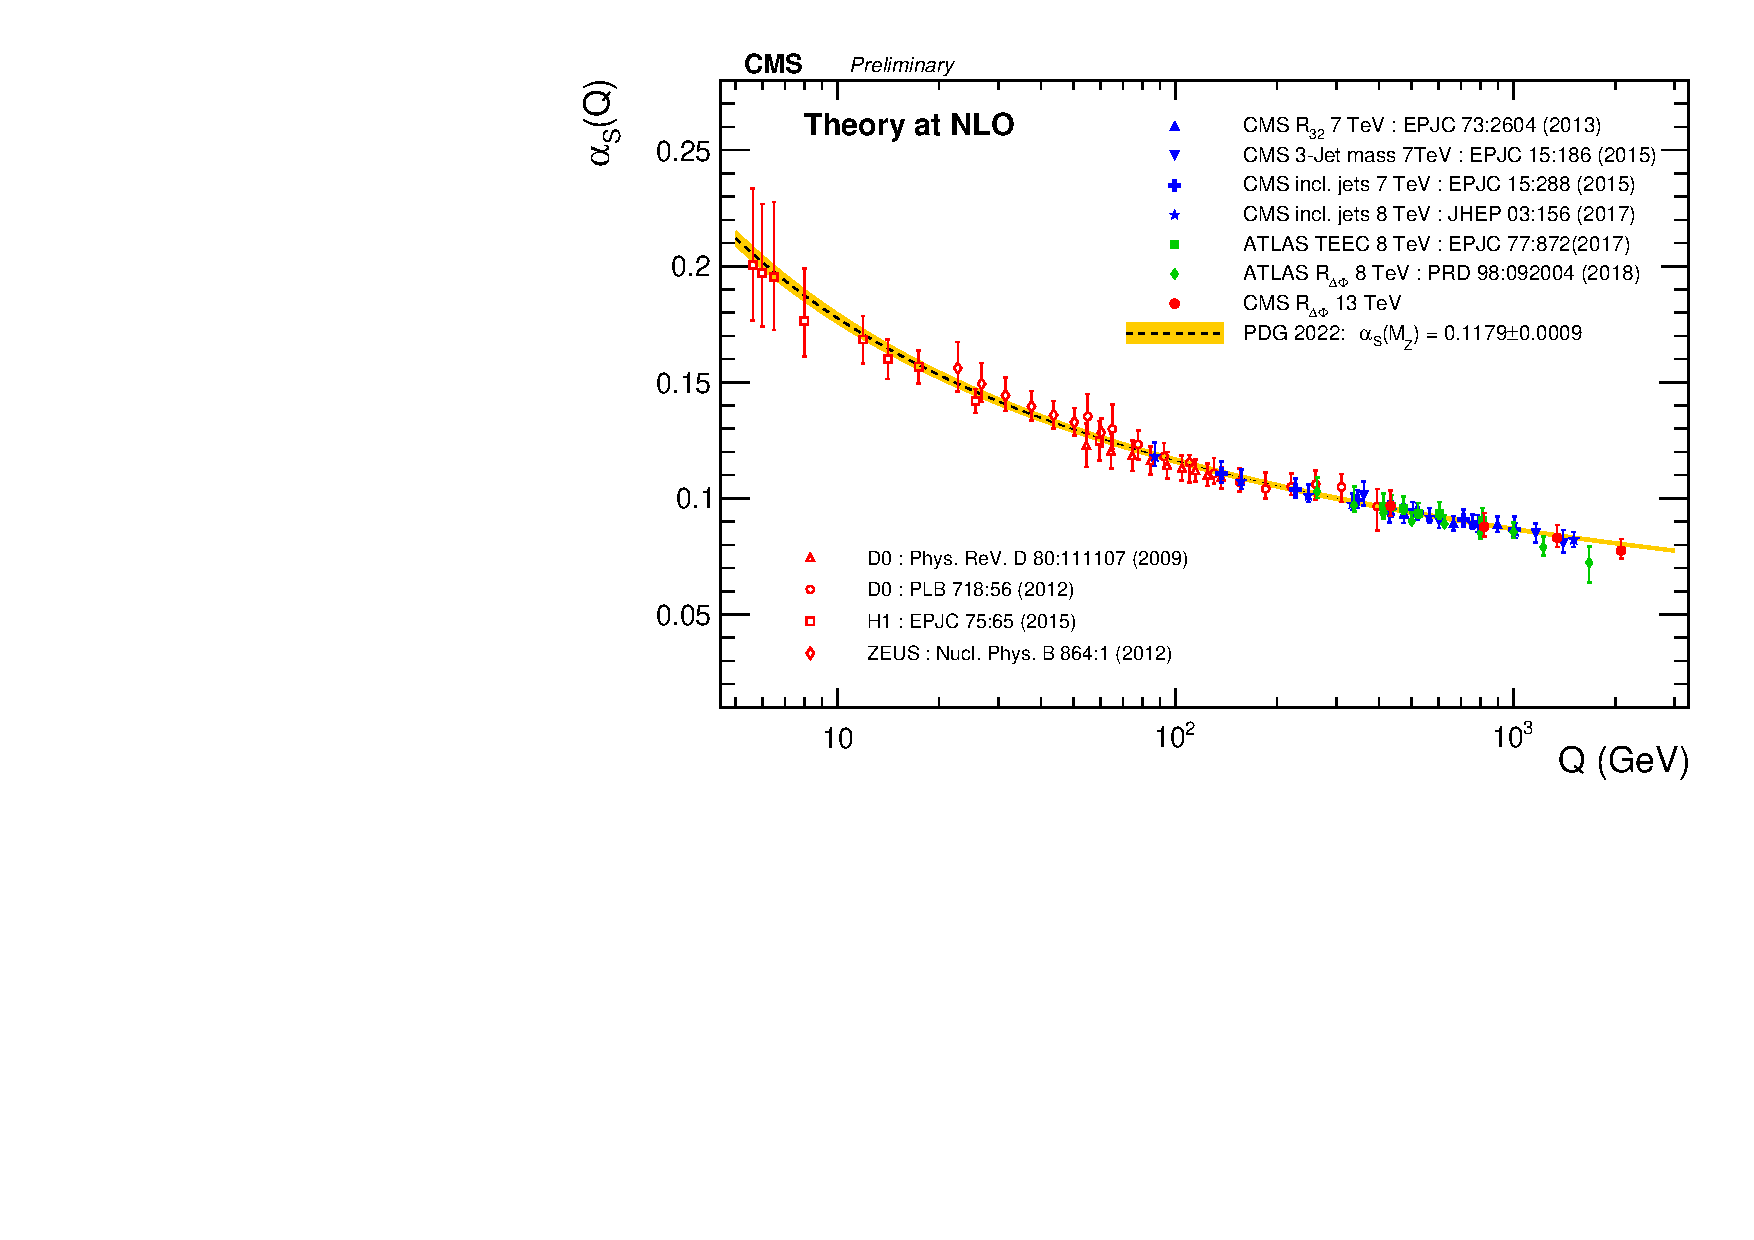
\includegraphics[width=0.8\textwidth]{figures/Part1/QCD/alphaS}
 \end{tabular}
 \caption{Summary of the running of $\alpha_{S}$ measured by \ac{CMS}, \ac{ATLAS} and other experiments. \cite{cms:twiki}}
 \label{fig:alphaS}
 \end{center}
\end{figure}

\section{Nonperturbative QCD and Hadron Collisions}
\label{sec:Collision}